\section[HGM]{Hierarchical Gaussian Mixtures}


\begin{frame}{Hierarchical Gaussian Mixtures}
\begin{block}
\justifying Let $\mathcal{U}, \mathcal{N}, \mathcal{W}$ be Uniform, Normal and Wishart distributions respectively. A Hierarchical Gaussian Mixture is then defined by:
\end{block}
\begin{center}
 \begin{minipage}{11cm}
 \begin{itemize}
    \item[F Features] %$F\in\mathbb{R}$
    \item[K classes] $C_k = (s_k, \Lambda_k, \nu_k, \Gamma_k) $ %with $s_k\in\mathbb{R}, \Lambda_k \in \mathbb{R}^{F\times F }, \nu_k\in \mathbb{R}^{F}, \Gamma_k\in \mathbb{R}^{F\times F})$
    \item[N datapoints] ($D_{n})_k = (\mu_n, \Sigma_n)_k$ with $\mu_n \sim \mathcal{N}(\nu_k ,\,\Gamma_k)$ and $\Sigma_n \sim \mathcal{W}(s_k, \,\Lambda_k)$
    \item[M Samples] $(S_{m})_n \sim \mathcal{N}(\mu_n,\,\Sigma_n)$
\end{itemize}
\end{minipage}
\end{center}
\begin{block}{For now:}
\justifying
 Random models with $F=2$ and hyperparameters $a,b \in \mathbb{R}_+$\\
 $s_k \sim \mathcal{U}([F,\infty])$, \quad $\nu_k \sim \mathcal{U}([-a,a]^F)$, \quad $\Gamma_k \sim \mathcal{W}(F, \,b\cdot\mathbb{1}_F)$, \quad and $\Lambda_k \sim \mathcal{W}(F, \,\mathbb{1}_F)$
\end{block}
\end{frame}


\subsection{Synthetic Data}

\begin{frame}{}
\begin{figure}
\includegraphics[height=\textheight]{HGM/RandomHGM.pdf}
\end{figure}
\end{frame}

\subsection{Wasserstein tSNE}

\begin{frame}{Wasserstein t-SNE}
\begin{block}{Formal Definition:}
\justifying
$W(\mu_{1}, \mu_{2})^{2} :=\left\|m_{1}-m_{2}\right\|_{2}^{2}+\text { trace }\left(C_{1}+C_{2}-2\left(C_{2}^{1 / 2} C_{1} C_{2}^{1 / 2}\right)^{1 / 2}\right)$
\end{block}

Now we introduce a hyperparameter $w \in [0,1]$, that puts emphasis either on means or covariances.

\begin{block}{Convex Generalization:}
\justifying
$W(\mu_{1}, \mu_{2})^{2} := (1-w) \cdot \left\|m_{1}-m_{2}\right\|_{2}^{2}+ w \cdot  \text { trace }\left(C_{1}+C_{2}-2\left(C_{2}^{1 / 2} C_{1} C_{2}^{1 / 2}\right)^{1 / 2}\right)$
\end{block}
\end{frame}



\begin{frame}{}
\begin{figure}
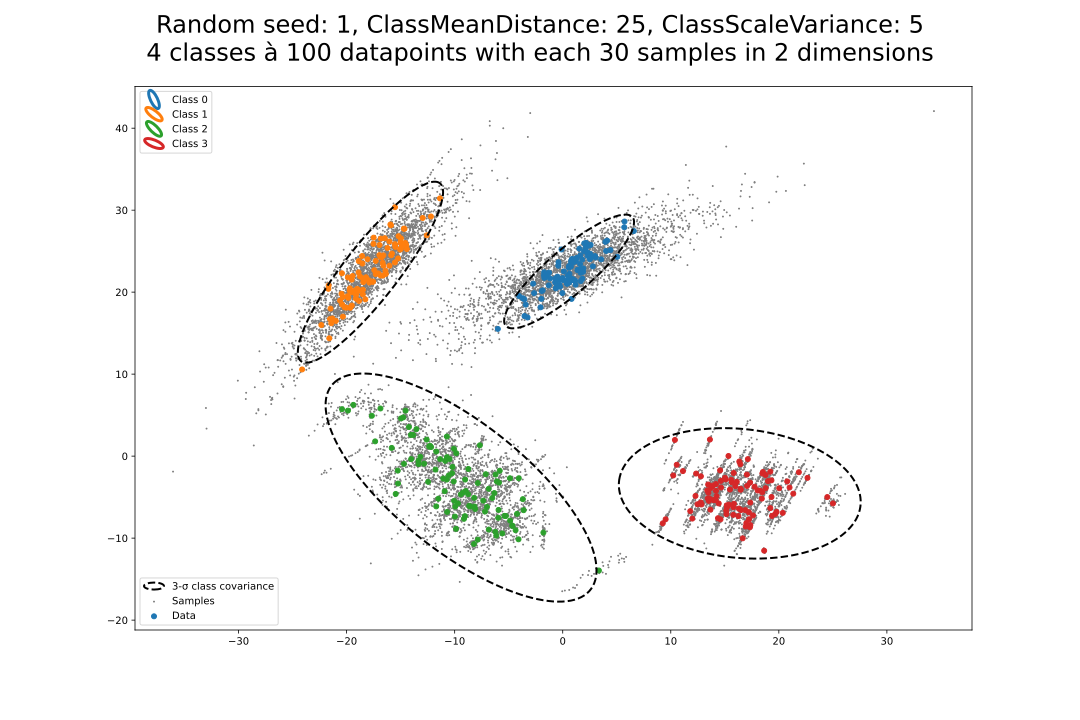
\includegraphics[width=\textwidth,height=\paperheight,keepaspectratio]{HGM/CleanExample}
\end{figure}
\end{frame}

\begin{frame}{}
\begin{figure}
\includegraphics[width=\textwidth]{HGM/RandomExample.pdf}
\end{figure}
\end{frame}

